\documentclass[12pt]{article}

\usepackage[margin=1in]{geometry}
\usepackage{amsfonts,amsmath,amssymb}
\usepackage{multicol}
\usepackage{graphicx}

\usepackage{float}
\usepackage[nottoc, notlot, notlof]{tocbibind}
\usepackage{hyperref}
\usepackage{enumitem}
\usepackage{caption}
\usepackage{subcaption}
\usepackage[T1]{fontenc}
%\usepackage[utf8]{inputenc}
\usepackage{xcolor}
\usepackage{pgfgantt}
\usepackage{rotating}
%\usepackage[graphicx]{realboxes}

\usepackage{color}
\definecolor{myblue}{rgb}{.8, .8, 1}
\definecolor{LightGray}{gray}{0.9}

\usepackage[most]{tcolorbox}
\tcbset{
	enhanced,
	colback=myblue!100!white,
	boxrule=0.1pt,
	colframe=myblue!100!black,
	fonttitle=\bfseries
}

\usepackage{minted} % For code 
\usepackage{tikz} % For checkmark



%\graphicspath{{/home/kushik/Kushik/VIT/Eighth semester/MagneticMirror/latex/forreport/Studies/}}

\def\checkmark{\tikz\fill[scale=0.5](0,.35) -- (.25,0) -- (1,.7) -- (.25,.15) -- cycle;} %define checkmark

\begin{document}

	\fontfamily{ppl}\selectfont 
	\begin{center}
		\Large{\textbf{Magnetic Mirror Effect in Magnetron Plasma:}} \\
		\Large{\textbf{Modeling of Plasma Parameters}} \\
	\end{center}
	
	\section{Checks}
	To verify that our program is working correctly, we perform some checks. We compare results from the program with calculations done by hand; of certain quantities and see if they agree. As of now, we are doing checks on the following aspects of the program:
	\begin{enumerate}
		\item Sampling \color{green} \checkmark \color{black}
		\item Update \color{green} \checkmark \color{black}
	\end{enumerate}
	
	\subsection{Sampling}
	As of now we our sampling of particle speeds is based on the Maxwell-Boltzmann distribution, that we have defined previously. We now check if the average speeds of the particles agrees with the calculations done by hand based on the plasma temperature.
	We recall the Maxwellian density function that we defined earlier. 
	\begin{equation}
		\label{eqn:maxwellian}
		\widehat{f_{M}} := \hat{f}(\boldsymbol{x}, \boldsymbol{v}, t) = \left(\frac{m}{2\pi KT}\right)^{\frac{3}{2}} \mathrm{exp}\left(-\frac{\boldsymbol{v}^{2}}{v_{th}^{2}}\right)
	\end{equation} where $$v_{th}^{2} = \frac{2 K T}{m}$$
	For our convenience, we use the density function with speed instead of velocity which is defined as:
	\begin{equation}
		\label{eqn:maxwellianSpeed}
		\widehat{f_{m}} := \hat{f}(\boldsymbol{x}, v, t) = \left(\frac{m}{2\pi KT}\right)^{\frac{3}{2}} 4 \pi v^{2} \: \mathrm{exp}\left(-\frac{v^{2}}{v_{th}^{2}}\right)
	\end{equation} which is obtained by integrating over the solid angle in the velocity variable. \\

	For this density function we calculate the average speed by with the expression:
	$$ \langle v\rangle = \int_{v = - \infty}^{v = \infty} d v \: v \: \widehat{f_{m}} = \int_{v = - \infty}^{v = \infty} d v \: v \: \left(\frac{m}{2\pi KT}\right)^{\frac{3}{2}} 4 \pi v^{2} \: \mathrm{exp}\left(-\frac{v^{2}}{v_{th}^{2}}\right)$$
	$$=  4 \pi \left(\frac{m}{2\pi KT}\right)^{\frac{3}{2}} \int_{v = - \infty}^{v = \infty} d v \: v^{3} \: \mathrm{exp}\left(-\frac{v^{2}}{v_{th}^{2}}\right)$$ $$ = 4 \pi \left(\frac{m}{2\pi KT}\right)^{\frac{3}{2}} \frac{v_{th}^{4}}{2} = 4 \pi \left(\frac{1}{\pi v_{th}^{2}}\right)^{\frac{3}{2}} \frac{v_{th}^{4}}{2}$$ $$= \frac{2}{\sqrt{\pi}} v_{th} = \frac{2}{\sqrt{\pi}} \sqrt{\frac{2 K T}{m}} = \frac{2}{\sqrt{\pi}} \sqrt{\frac{2 R T}{M}}$$ 
	For the Hydrogen atom particle distribution, we get \begin{tcolorbox}
		$$\langle v\rangle = \frac{2}{\sqrt{\pi}} \sqrt{\frac{2 \cdot 8.31446261815324 \: \mathrm{J} \: \mathrm{K}^{-1} \: \mathrm{mol}^{-1} \: 10000 \: \mathrm{K}}{1.008 \times 10^{-3} \: \mathrm{kg} \: \mathrm{mol}^{-1}}} = 14492.952993825973 \: \mathrm{m}\mathrm{s}^{-1}$$
	\end{tcolorbox}
	
	From section 1.1.1 Maxwellian sampling in the \textbf{checks.ipynb} notebook, we take the following:
	
	\begin{center}
		\begin{tcolorbox}[width=3.5cm]
			Initialization
		\end{tcolorbox}
	\end{center}
	\begin{minted}[
		frame=lines,
		framesep=2mm,
		baselinestretch=1.2,
		bgcolor=LightGray,
		fontsize=\footnotesize,
		linenos=true,
		breaklines
		]
		{python}
# c1Maxwell means checking the Maxwellian sampling
c1Maxwell = Run()
# Create 100 particles based on the data available in the files
c1Maxwell.create_batch_with_file_initialization('H+', constants.constants['e'][0], constants.constants['m_H'][0] * constants.constants['amu'][0], 100, 100, 'H ions', r_index=0, v_index=1)	
	\end{minted}
	\begin{center}
		\begin{tcolorbox}[width=3cm]
			Inspection
		\end{tcolorbox}
	\end{center}
	\begin{minted}[
		frame=lines,
		framesep=2mm,
		baselinestretch=1.2,
		bgcolor=LightGray,
		fontsize=\footnotesize,
		linenos=true,
		breaklines
		]
		{python}
# Take the 0th batch of particles
c1Maxwell_batch = c1Maxwell.batches[0]['H ions']
# Take the initial positions and velocities of the particles
c1Maxwell_positions = []
c1Maxwell_velocities = []
for particle in c1Maxwell_batch.particles:
c1Maxwell_positions.append(particle.r)
c1Maxwell_velocities.append(particle.v)
# Let's now look at the velocities
c1Maxwell_velocities
# We need to check if they are really Maxwellian distributed
# Get the speeds 
c1Maxwell_speeds = np.sqrt( [ (c1Maxwell_velocities[i][0] ** 2) + (c1Maxwell_velocities[i][1] ** 2) + (c1Maxwell_velocities[i][2] ** 2) for i in range(len(c1Maxwell_velocities)) ] )
c1Maxwell_meanspeed = np.sum(c1Maxwell_speeds) / c1Maxwell_speeds.size	
	\end{minted}
We get an average speed of the distribution to be:
\begin{tcolorbox}
	\begin{verbatim}
	14202.764572898674
\end{verbatim}
\end{tcolorbox}

We see that the mean average speed of the sampled distribution and that expected from the analytic expression are close; in fact within $2.0431826454479785 \%$ error.

To be confident that our program indeed samples particles based on Maxwellian distribution as we expect it to, let's check another distribution. For convenience, let's assume Hydrogen molecules to be particles sampled with Maxwellian distribution, and check if the average speed of the sampled distribution agrees with the that expected from analytic calculation. For this we follow a similar procedure.

\begin{center}
	\begin{tcolorbox}[width=3.5cm]
		Initialization
	\end{tcolorbox}
\end{center}
\begin{minted}[
	frame=lines,
	framesep=2mm,
	baselinestretch=1.2,
	bgcolor=LightGray,
	fontsize=\footnotesize,
	linenos=true,
	breaklines
	]
	{python}
# Create 100 particles based on the sampled velocities of H2 gas
# We consider just for this test case that a Hydrogen molecules to be sampled with a Maxwellian distribution
# We create a new batch on the same Run instance
c1Maxwell.create_batch_with_file_initialization('H2', constants.constants['e'][0], 2 * constants.constants['m_H'][0] * constants.constants['amu'][0], 100, 100, 'H2 gas', r_index=0, v_index=2)	
\end{minted}
\begin{center}
	\begin{tcolorbox}[width=3cm]
		Inspection
	\end{tcolorbox}
\end{center}
\begin{minted}[
	frame=lines,
	framesep=2mm,
	baselinestretch=1.2,
	bgcolor=LightGray,
	fontsize=\footnotesize,
	linenos=true,
	breaklines
	]
	{python}
# Do the same as before for the second batch
c1Maxwell_batch2 = c1Maxwell.batches[1]['H2 gas']
c1Maxwell_positions_batch2 = []
c1Maxwell_velocities_batch2 = []
for particle in c1Maxwell_batch2.particles:
c1Maxwell_positions_batch2.append(particle.r)
c1Maxwell_velocities_batch2.append(particle.v)
c1Maxwell_speeds_batch2 = np.sqrt( [ (c1Maxwell_velocities_batch2[i][0] ** 2) + (c1Maxwell_velocities_batch2[i][1] ** 2) + (c1Maxwell_velocities_batch2[i][2] ** 2) for i in range(len(c1Maxwell_velocities_batch2)) ] )
c1Maxwell_meanspeed_batch2 = np.sum(c1Maxwell_speeds_batch2) / c1Maxwell_speeds_batch2.size	
\end{minted}

We get an average speed of the distribution to be:
\begin{tcolorbox}
	\begin{verbatim}
		10149.754879907316
	\end{verbatim}
\end{tcolorbox}

	For the Hydrogen molecule particle distribution, we get \begin{tcolorbox}
	$$\langle v\rangle = \frac{2}{\sqrt{\pi}} \sqrt{\frac{2 \cdot 8.31446261815324 \: \mathrm{J} \: \mathrm{K}^{-1} \: \mathrm{mol}^{-1} \: 10000 \: \mathrm{K}}{2 \times 1.008 \times 10^{-3} \: \mathrm{kg} \: \mathrm{mol}^{-1}}} = 10248.06534135222 \: \mathrm{m}\mathrm{s}^{-1}$$
\end{tcolorbox}

We see that the mean average speed of the sampled distribution and that expected from the analytic expression are close for this distribution too; in fact within $0.9685993662716086 \%$ error. Because the errors are considerably small compared to statistical variation in the sampling, we believe the Maxwellian distribution sampling part of the program to be working as we expect it to.

	\subsection{Update}
		We recall the Boris Algorithm, that we use to update the particles in the plasma simulation.
		\begin{center}
			\begin{tcolorbox}[width=8cm]
				
				\begin{equation}
					\label{Boris Algorithm}
					\begin{split}
						\boldsymbol{v}^{-} & = \boldsymbol{v}_{k} + q^{\prime} \mathbf{E}_{k} \\
						\boldsymbol{v}^{+} & = \boldsymbol{v}^{-} + 2 q^{\prime} \left( \boldsymbol{v}^{-} \times \mathbf{B}_{k} \right) \\
						\boldsymbol{v}_{k+1} & = \boldsymbol{v}^{+} + q^{\prime} \mathbf{E}_{k} \\
						\boldsymbol{x}_{k+1} & = \boldsymbol{x}_{k} + \Delta t \hspace{0.2cm}\boldsymbol{v}_{k+1}
					\end{split}	 			
				\end{equation}
			\end{tcolorbox}
		\end{center}
		where $q^{\prime} = \frac{\displaystyle q}{\displaystyle m} \frac{\displaystyle \Delta t}{ 2}$.
		
		To verify that the simulation works as we expect it to, we perform a calculation and compare it to the output of an algorithm. From section 1.2.1 Boris Update in the \textbf{checks.ipynb} notebook, we take the following:
		\begin{center}
			\begin{tcolorbox}[width=3.5cm]
				Initialization
			\end{tcolorbox}
		\end{center}

		\begin{minted}[
			frame=lines,
			framesep=2mm,
			baselinestretch=1.2,
			bgcolor=LightGray,
			fontsize=\footnotesize,
			linenos=true,
			breaklines
			]
			{python}
# c2Boris means checking the Boris update
c2Boris = Run()
#Create 10 particles
c2Boris.create_batch_with_file_initialization('H+', constants.constants['e'][0], constants.constants['m_H'][0] * constants.constants['amu'][0], 100, 10, 'H ions', r_index=0, v_index=1)		
		\end{minted}
		\begin{center}
			\begin{tcolorbox}[width=4.5cm]
				Update input data
			\end{tcolorbox}
		\end{center}		

		\begin{minted}[
			frame=lines,
			framesep=2mm,
			baselinestretch=1.2,
			bgcolor=LightGray,
			fontsize=\footnotesize,
			linenos=true,
			breaklines
			]
			{python}
											
c2Boris_index_update = 0 # Update the first batch in this Run instance run_Boris_check
c2Boris_particle_track_indices = [i for i in range(10)] # Track all 10 particles
c2Boris_dT = 10**(-6) # 1 microseconds
c2Boris_stepT = 10**(-7) # 0.1 microseconds time step
c2Boris_E0 = 1000 # say 1000 Volts (voltage) per meter (size of chamber) 
c2Boris_Edirn = [1,0,0] #in the x-direction [1,0,0]
c2Boris_B0 = 10 * (10**(-3)) # Meant to say 10 mT 
c2Boris_Bdirn = [0,1,0] #in the y-direction [0,1,0]
c2Boris_argsE = [element * c2Boris_E0 for element in c2Boris_Edirn] # currently the uniform_E_field configuration is used
c2Boris_argsB = [element * c2Boris_B0 for element in c2Boris_Bdirn]# currently the uniform_B_field configuration is used
		\end{minted}
	
		\begin{center}
		\begin{tcolorbox}[width=2.5cm]
			Update
		\end{tcolorbox}
		\end{center}
	
	\begin{minted}[
		frame=lines,
		framesep=2mm,
		baselinestretch=1.2,
		bgcolor=LightGray,
		fontsize=\footnotesize,
		linenos=true,
		breaklines,
		]          
		{python}
c2Boris_positions_and_velocities = c2Boris.update_batch_with_unchanging_fields(c2Boris_index_update, c2Boris_dT, c2Boris_stepT, c2Boris_argsE, c2Boris_argsB, c2Boris_particle_track_indices)	

#Let's inspect the positions and velocities of the particles at index 1 and 7
c2Boris_p1 = c2Boris_positions_and_velocities[1]
c2Boris_p7 = c2Boris_positions_and_velocities[7]

#Let's take the positions and velocities of the particle 1 after the 3rd and the 4th time steps.
c2Boris_p134_p = [c2Boris_p1[3][1], c2Boris_p1[4][1]]
c2Boris_p134_v = [c2Boris_p1[3][2], c2Boris_p1[4][2]]

#Similary for particle 7
c2Boris_p734_p = [c2Boris_p7[3][1], c2Boris_p7[4][1]]
c2Boris_p734_v = [c2Boris_p7[3][2], c2Boris_p7[4][2]]	
	\end{minted}
The program gives the following output. For example, we can check the particles 1 and 7 in the update. After the $3^{rd}$ step of the update, the velocity of particle 1 was:
\begin{tcolorbox}
	\begin{verbatim}
		[39771.83801956555, -5029.491038, 4533.343932509505]
	\end{verbatim}
\end{tcolorbox}
and after the $4^{th}$ update, it changed to:
\begin{tcolorbox}
	\begin{verbatim}
	[48909.86581773698, -5029.491038, 8798.399243869582]
\end{verbatim}
\end{tcolorbox}
Its position after the $3^{rd}$ step of the update was:
\begin{tcolorbox}
	\begin{verbatim}
	[-0.48985112694809785, -0.0020117964152, 0.00017005183797547688]
\end{verbatim}
\end{tcolorbox}
which was updated after the $4^{th}$ step of the update to:
\begin{tcolorbox}
	\begin{verbatim}
[-0.4849601403663242, -0.0025147455189999997, 0.001049891762362435] 
\end{verbatim}
\end{tcolorbox}
We now check if the same if true, with a calculation of the update done by hand.
$$q^{\prime} = \frac{\displaystyle q}{\displaystyle m} \frac{\displaystyle \Delta t}{ 2} = \frac{\displaystyle 1.602176634 \times 10^{-19} \: \mathrm{C}} {\displaystyle 1.008 \: \mathrm{a.m.u.} \times 1.6605390666 \times 10^{-27} \: \mathrm{kg} \: \mathrm{a.m.u.}^{-1}} \frac{\displaystyle 10^{-7} \: \mathrm{s}}{ 2} = 4.78597877761177 \: \mathrm{C} \: \mathrm{s} \: \mathrm{kg}^{-1}$$

$\boldsymbol{v}^{-} = \boldsymbol{v}_{3} + q^{\prime} \mathbf{E} = \begin{bmatrix} 
	39771.83801956555 \\ -5029.491038 \\ 4533.343932509505
\end{bmatrix} + 4.78597877761177 \begin{bmatrix}
 1000 \\ 0 \\ 0 
\end{bmatrix} = \begin{bmatrix}
44557.81679718 \\ -5029.491038 \\  4533.34393251
\end{bmatrix}$
$$\boldsymbol{v}^{+} = \boldsymbol{v}^{-} + 2 q^{\prime} \left( \boldsymbol{v}^{-} \times \mathbf{B} \right) = \begin{bmatrix}
	44557.81679718 \\ -5029.491038 \\  4533.34393251
\end{bmatrix} + 2 \cdot 4.78597877761177 \left( \begin{bmatrix}
44557.81679718 \\ -5029.491038 \\  4533.34393251
\end{bmatrix} \times \begin{bmatrix}
0.0 \\ 0.01 \\ 0.0
\end{bmatrix} \right)$$ $$ = \begin{bmatrix}
44123.88704013 \\ -5029.491038 \\ 8798.39924387
\end{bmatrix}$$
\begin{tcolorbox}
	$$\boldsymbol{v}_{4} = \boldsymbol{v}^{+} + q^{\prime} \mathbf{E} = \begin{bmatrix}
	44123.88704013 \\ -5029.491038 \\ 8798.39924387
\end{bmatrix} + 4.78597877761177 \begin{bmatrix}
1000 \\ 0 \\ 0 
\end{bmatrix} = \begin{bmatrix}
48909.86581774 \\ -5029.491038 \\  8798.39924387
\end{bmatrix}$$
\end{tcolorbox}
\begin{tcolorbox}
	$$\boldsymbol{x}_{4} = \boldsymbol{x}_{3} + \Delta t \hspace{0.2cm}\boldsymbol{v}_{4} = \begin{bmatrix}
	-4.89851127 \times 10^{-01} \\ -2.01179642\times 10^{-03} \\  1.70051838\times 10^{-04}
\end{bmatrix} + 10^{-7} \hspace{0.2cm}\ \begin{bmatrix}
48909.86581774 \\ -5029.491038 \\  8798.39924387
\end{bmatrix} = \begin{bmatrix}
-0.48496014 \\ -0.00251475 \\  0.00104989
\end{bmatrix}$$
\end{tcolorbox}
We see that the values for $\boldsymbol{x_{3}}$, $\boldsymbol{x_{4}}$, $\boldsymbol{v_{3}}$ and $\boldsymbol{v_{4}}$ for particle 1 are close (the latter digits differ due to the differing precision of calculations); i.e. the same when done by hand and in the program.

\noindent Similarly, for particle 7. After the $3^{rd}$ step of the update, the velocity of the particle was:
\begin{tcolorbox}
	\begin{verbatim}
[38895.85871094631, -8670.854777, 13914.969423620274]
\end{verbatim}
\end{tcolorbox}
and after the $4^{th}$ update, it changed to:
\begin{tcolorbox}
	\begin{verbatim}
[47135.881299118584, -8670.854777, 18096.176367366777]
\end{verbatim}
\end{tcolorbox}
Its position after the $3^{rd}$ step of the update was:
\begin{tcolorbox}
	\begin{verbatim}
[-0.4896669752432719, -0.0034683419108, 0.0038875496903932644] 
\end{verbatim}
\end{tcolorbox}
which was updated after the $4^{th}$ step of the update to:
\begin{tcolorbox}
	\begin{verbatim}
[-0.48495338711336006, -0.0043354273885, 0.0056971673271299424]
\end{verbatim}
\end{tcolorbox}

$\boldsymbol{v}^{-} = \boldsymbol{v}_{3} + q^{\prime} \mathbf{E} = \begin{bmatrix} 
	 38895.85871095 \\ -8670.854777 \\ 13914.96942362
\end{bmatrix} + 4.78597877761177 \begin{bmatrix}
	1000 \\ 0 \\ 0 
\end{bmatrix} = \begin{bmatrix}
	43681.83748856 \\ -8670.854777 \\ 13914.96942362
\end{bmatrix}$
$$\boldsymbol{v}^{+} = \boldsymbol{v}^{-} + 2 q^{\prime} \left( \boldsymbol{v}^{-} \times \mathbf{B} \right) = \begin{bmatrix}
	43681.83748856 \\ -8670.854777 \\ 13914.96942362
\end{bmatrix} + 2 \cdot 4.78597877761177 \left( \begin{bmatrix}
	43681.83748856 \\ -8670.854777 \\ 13914.96942362
\end{bmatrix} \times \begin{bmatrix}
	0.0 \\ 0.01 \\ 0.0
\end{bmatrix} \right)$$ $$ = \begin{bmatrix}
	42349.90252151 \\ -8670.854777  \\ 18096.17636737
\end{bmatrix}$$
\begin{tcolorbox}
	$$\boldsymbol{v}_{4} = \boldsymbol{v}^{+} + q^{\prime} \mathbf{E} = \begin{bmatrix}
	42349.90252151 \\ -8670.854777  \\ 18096.17636737
\end{bmatrix} + 4.78597877761177 \begin{bmatrix}
	1000 \\ 0 \\ 0 
\end{bmatrix} = \begin{bmatrix}
	47135.88129912 \\ -8670.854777 \\ 18096.17636737
\end{bmatrix}$$
\end{tcolorbox}
\begin{tcolorbox}
	$$\boldsymbol{x}_{4} = \boldsymbol{x}_{3} + \Delta t \hspace{0.2cm}\boldsymbol{v}_{4} = \begin{bmatrix}
	-0.48966698 \\ -0.00346834 \\  0.00388755
\end{bmatrix} + 10^{-7} \hspace{0.2cm}\ \begin{bmatrix}
	47135.88129912 \\ -8670.854777 \\ 18096.17636737
\end{bmatrix} = \begin{bmatrix}
	-0.48495339 \\ -0.00433543 \\  0.00569717
\end{bmatrix}$$
\end{tcolorbox}
We see that the values for $\boldsymbol{x_{3}}$, $\boldsymbol{x_{4}}$, $\boldsymbol{v_{3}}$ and $\boldsymbol{v_{4}}$ for particle 7 are close (the latter digits differ due to the differing precision of calculations); i.e. the same when done by hand and in the program.	

Based on these calculations, we believe that our particle update works as expected; according to the Boris Algorithm, and this part of the program works correctly. 
		
	\section{Plasma Stream}
	We now create our first plasma system, where we can change certain parameters of the fields; so as to simulate controlling plasma in a chamber by changing the electric and magnetic fields as required. We discuss the program written in \textbf{study1.ipynb}.
	
	\subsection{Setup}
	
	After making the imports, we first create the system as in a batch of particle of a run object instance.
	\begin{minted}[
		frame=lines,
		framesep=2mm,
		baselinestretch=1.2,
		bgcolor=LightGray,
		fontsize=\footnotesize,
		linenos=true,
		breaklines
		]
		{python}
#Create a constants object instance to access the constants from constants.ipynb file
constants = Constants()
# Create a run object instance
s1 = Run()
# Create 100 Hydrogen ions whose:
# speeds are Maxwellian sampled, velocity directions are uniform randomly sampled
# positions are all sampled such that particles start at [-0.5, 0, 0] 
# a chamber 1m x 1m x 1m with extreme points [-0.5, -0.5, -0.5] and [0.5, 0.5, 0.5] considered
s1.create_batch_with_file_initialization('H+', constants.constants['e'][0], constants.constants['m_H'][0] * constants.constants['amu'][0], 100, 100, 'H ions', r_index=0, v_index=1)	
	\end{minted}
	
	After creating a batch of particle, we take that batch and update it under the action of Electric and Magnetic fields.	Here we consider constant magnetic field of 10 mT along the $y$-axis [0,1,0] and changing electric field configurations of [0, 0, 1, -1, 2, -2, 3, -3, 4, -4, 5, -5] $\times$ 1000 V$\mathrm{m}^{-1}$ along the $x$-axis [1,0,0]. For a time duration of 0.1 ms we update the batch of particles under different configurations of the electric field, using time steps of 0.001 ms and get the positions and velocities of the particles during the history of updates.
\begin{minted}[
	frame=lines,
	framesep=2mm,
	baselinestretch=1.2,
	bgcolor=LightGray,
	fontsize=\footnotesize,
	linenos=true,
	breaklines
	]
	{python}
# Take the first batch in this run object
s1_batch1 = s1.batches[0]['H ions']

# Let's consider Electric field being flipped in direction, and taken up a few scales
E_scale = [0, 0, 1, -1, 2, -2, 3, -3, 4, -4, 5, -5]
# Let's consider a case with constant Magnetic field
B_scale = [1 for i in range(len(E_scale))]

s1_index_update = 0 # Update the first batch in this Run instance 
s1_particle_track_indices = [i for i in range(100)] # Track all 100 particles
s1_dT = 10**(-7) # 0.1 microseconds
s1_stepT = 10**(-9) # 0.001 microseconds time step
s1_E0 = 1000 # say 1000 Volts (voltage) per meter (size of chamber) 
s1_Edirn = [1,0,0] #in the x-direction [1,0,0]
s1_B0 = 10 * (10**(-3)) # Meant to say 10 mT 
s1_Bdirn = [0,1,0] #in the y-direction [0,1,0]

s1_argsE = [element * s1_E0 for element in s1_Edirn] # currently the uniform_E_field configuration is used
s1_argsB = [element * s1_B0 for element in s1_Bdirn] # currently the uniform_B_field configuration is used

s1_batch_ps_and_vs = dict()

for i in range(len(E_scale)):
	desc = 'E_scale = ' + str(E_scale[i]) + ' ' + 'B_scale = ' + str(B_scale[i])
	s1_batch1_ps_and_vs_once = s1.update_batch_with_unchanging_fields(s1_index_update, s1_dT, s1_stepT, [elem *E_scale[i] for elem in s1_argsE], [elem *E_scale[i] for elem in s1_argsB] * B_scale[i], s1_particle_track_indices)
	s1_batch_ps_and_vs[desc] = s1_batch1_ps_and_vs_once 
\end{minted}

	Now we need to extract and arrange the positions and velocities of the particles during the update history and plot them. Let's first look at the particle at index 0. Let's first extract the position and velocities of particle zero when the electric field was scaled by +1 and -1 and plot the positions.
	
	
\begin{minted}[
	frame=lines,
	framesep=2mm,
	baselinestretch=1.2,
	bgcolor=LightGray,
	fontsize=\footnotesize,
	linenos=true,
	breaklines
	]
	{python}
s1_descE_is_1 = 'E_scale = ' + str(E_scale[2]) + ' ' + 'B_scale = ' + str(B_scale[2])
s1_descE_is_n1 = 'E_scale = ' + str(E_scale[3]) + ' ' + 'B_scale = ' + str(B_scale[3])
# Extract update histories for two field configs
s1_histories_E1 = s1_batch_ps_and_vs[s1_descE_is_1]
s1_histories_nE1 = s1_batch_ps_and_vs[s1_descE_is_n1]

# Extract information on 0th particle's update history in both cases
s1_descE_is_1_p0 = s1_histories_E1[0]
s1_descE_is_n1_p0 =  s1_histories_nE1[0]

#Get positions and velocities of the particle's update history
s1_descE_is_1_p0_ps = []
s1_descE_is_1_p0_vs = []

for i in range(len(s1_descE_is_1_p0)):
	s1_descE_is_1_p0_ps.append(s1_descE_is_1_p0[i][1])
	s1_descE_is_1_p0_vs.append(s1_descE_is_1_p0[i][2])
	
	s1_descE_is_n1_p0_ps = []
	s1_descE_is_n1_p0_vs = []

for i in range(len(s1_descE_is_n1_p0)):
	s1_descE_is_n1_p0_ps.append(s1_descE_is_n1_p0[i][1])
	s1_descE_is_n1_p0_vs.append(s1_descE_is_n1_p0[i][2])
\end{minted}

	Now we plot the positions of the particle at index 0 when the electric field was scaled by +1 and -1.
	
\begin{minted}[
	frame=lines,
	framesep=2mm,
	baselinestretch=1.2,
	bgcolor=LightGray,
	fontsize=\footnotesize,
	linenos=true,
	breaklines
	]
	{python}
# Plot the position update history of particle 0 when the electric field is scaled by 1
s1_descE_is_1_p0_ps_fig = plt.figure()
s1_descE_is_1_p0_ps_ax = plt.axes(projection='3d')
s1_descE_is_1_p0_ps_ax.view_init(50, -20)

# Data for three-dimensional scattered points
# for position update history of particle 0 when the Electric field was scaled by 1
s1_descE_is_1_p0_ps_zdata = [elem[2] for elem in s1_descE_is_1_p0_ps]
s1_descE_is_1_p0_ps_xdata = [elem[0] for elem in s1_descE_is_1_p0_ps]
s1_descE_is_1_p0_ps_ydata = [elem[1] for elem in s1_descE_is_1_p0_ps]
s1_descE_is_1_p0_ps_ax.scatter3D(s1_descE_is_1_p0_ps_xdata, s1_descE_is_1_p0_ps_ydata, s1_descE_is_1_p0_ps_zdata,\
c=s1_descE_is_1_p0_ps_zdata, cmap='Greens');
plt.savefig('EplusPs', dpi='figure', format='png')

# Plot the position update history of particle 0 when the electric field is scaled by -1
# We see an opposite curve to the previous figure
s1_descE_is_n1_p0_ps_fig = plt.figure()
s1_descE_is_n1_p0_ps_ax = plt.axes(projection='3d')
s1_descE_is_n1_p0_ps_ax.view_init(50, -20)

# Data for three-dimensional scattered points
# for position update history of particle 0 when the Electric field was scaled by -1
s1_descE_is_n1_p0_ps_zdata = [elem[2] for elem in s1_descE_is_n1_p0_ps]
s1_descE_is_n1_p0_ps_xdata = [elem[0] for elem in s1_descE_is_n1_p0_ps]
s1_descE_is_n1_p0_ps_ydata = [elem[1] for elem in s1_descE_is_n1_p0_ps]
s1_descE_is_n1_p0_ps_ax.scatter3D(s1_descE_is_n1_p0_ps_xdata, s1_descE_is_n1_p0_ps_ydata, \
s1_descE_is_n1_p0_ps_zdata, c=s1_descE_is_n1_p0_ps_zdata, cmap='Greens');
plt.savefig('EminusPs', dpi='figure', format='png')
\end{minted}

The plots output are as following. All numbers are in meters. In 3-dimensional plots, the vertical axis represents the $z$-axis, the axis into the page of the plane represents the $x$-axis and the axis along the lines the page represents the $y$-axis. In 1 dimensional plots, the vertical axis represents the value being plotted and the horizontal axis represents the steps of iteration.


\begin{figure}[H]
	\begin{multicols}{2}
		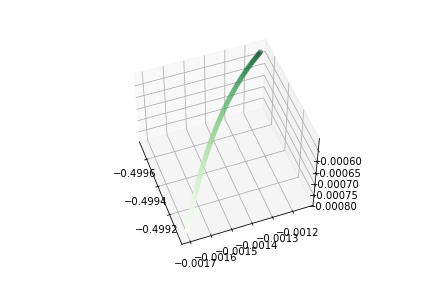
\includegraphics[width=\linewidth, height=6cm]{EplusPs1.png} \caption{Electric field scaled by 1} \par
		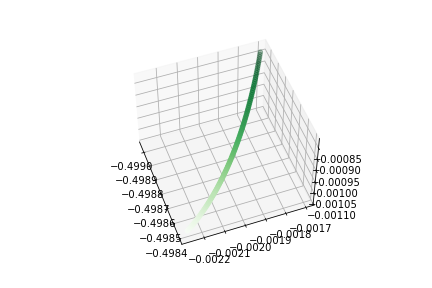
\includegraphics[width=\linewidth, height=6cm]{EminusPs1.png} \caption{Electric field scaled by -1} \par
	\end{multicols}
\end{figure}

	\subsection{Plotting particle update history}
	One can notice that the particle seems to curve differently. To make things more clear, let's plot the position of the particle during all of the used configurations of the electric field. 
	
\begin{minted}[
	frame=lines,
	framesep=2mm,
	baselinestretch=1.2,
	bgcolor=LightGray,
	fontsize=\footnotesize,
	linenos=true,
	breaklines
	]
	{python}
# take for a field configuration
s1_allFieldkeys = list(s1_batch_ps_and_vs.keys())
s1_allfield_p0_ps = []
s1_allfield_p0_vs = []
for akey in s1_allFieldkeys:
s1_histories = s1_batch_ps_and_vs[akey]

#Take particle 0
s1_p0 = s1_histories[0]

#Take ps and vs
for i in range(len(s1_p0)):
	s1_allfield_p0_ps.append(s1_p0[i][1])
	s1_allfield_p0_vs.append(s1_p0[i][2])
	s1_allfield_p0_ps = np.array(s1_allfield_p0_ps)
	s1_allfield_p0_vs = np.array(s1_allfield_p0_vs)

#Plot the position
s1_allfield_p0_ps_fig = plt.figure()
s1_allfield_p0_ps_ax = plt.axes(projection='3d')
s1_allfield_p0_ps_ax.view_init(20, -50)

# Data for three-dimensional scattered points
# for position update history of particle 0 during all field configurations
s1_allfield_p0_ps_zdata = [elem[2] for elem in s1_allfield_p0_ps]
s1_allfield_p0_ps_xdata = [elem[0] for elem in s1_allfield_p0_ps]
s1_allfield_p0_ps_ydata = [elem[1] for elem in s1_allfield_p0_ps]
s1_allfield_p0_ps_ax.scatter3D(s1_allfield_p0_ps_xdata, s1_allfield_p0_ps_ydata, s1_allfield_p0_ps_zdata,\
c=s1_allfield_p0_ps_zdata, cmap='Greens');
plt.savefig('ps1', dpi='figure', format='png')
\end{minted}
	
	We also plot the $x$, $y$ and $z$ components of position during the evolution, against the update steps.	

\begin{minted}[
	frame=lines,
	framesep=2mm,
	baselinestretch=1.2,
	bgcolor=LightGray,
	fontsize=\footnotesize,
	linenos=true,
	breaklines
	]
	{python}
# Plot x position
s1_allfield_p0_ps_x_fig = plt.figure()
s1_allfield_p0_ps_x_ax = plt.axes()
s1_allfield_p0_ps_x_ax.scatter(np.arange(len(s1_allfield_p0_ps_xdata)), s1_allfield_p0_ps_xdata);
plt.savefig('psx1', dpi='figure', format='png')

# Plot y position
s1_allfield_p0_ps_y_fig = plt.figure()
s1_allfield_p0_ps_y_ax = plt.axes()
s1_allfield_p0_ps_y_ax.scatter(np.arange(len(s1_allfield_p0_ps_ydata)), s1_allfield_p0_ps_ydata);
plt.savefig('psy1', dpi='figure', format='png')

# Plot z position
s1_allfield_p0_ps_z_fig = plt.figure()
s1_allfield_p0_ps_z_ax = plt.axes()
s1_allfield_p0_ps_z_ax.scatter(np.arange(len(s1_allfield_p0_ps_zdata)), s1_allfield_p0_ps_zdata);
plt.savefig('psz1', dpi='figure', format='png')
\end{minted}

We get the following figures for the position and its components for the particle during the update.

\begin{figure}[H]
	\begin{multicols}{2}
		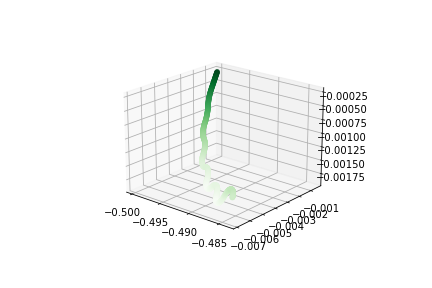
\includegraphics[width=\linewidth, height=6cm]{ps1.png} \caption{position} \label{ps1} \par
		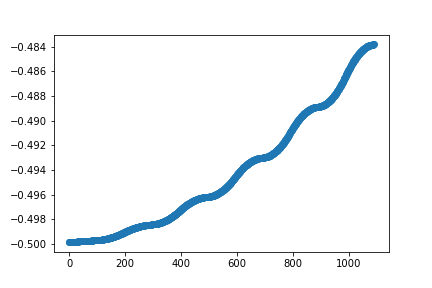
\includegraphics[width=\linewidth, height=6cm]{psx1.png} \caption{$x$-component of position} \label{psx1} \par
	\end{multicols}
\end{figure}
\begin{figure}[H]
	\begin{multicols}{2}
		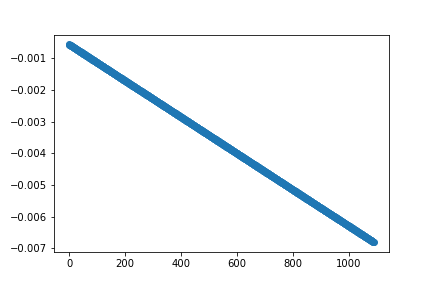
\includegraphics[width=\linewidth, height=6cm]{psy1.png} \caption{$y$-component of position} \label{psy1} \par
		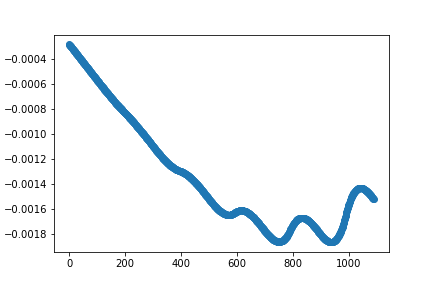
\includegraphics[width=\linewidth, height=6cm]{psz1.png} \caption{$z$-component of position} \label{psz1} \par
	\end{multicols}
\end{figure}

	We also plot the velocity and components of velocity of the particle.

\begin{minted}[
	frame=lines,
	framesep=2mm,
	baselinestretch=1.2,
	bgcolor=LightGray,
	fontsize=\footnotesize,
	linenos=true,
	breaklines
	]
	{python}
# Plot the velocity
s1_allfield_p0_vs_fig = plt.figure()
s1_allfield_p0_vs_ax = plt.axes(projection='3d')
s1_allfield_p0_vs_ax.view_init(20, -80)

# Data for three-dimensional scattered points
# for position update history of particle 0 during all field configurations
s1_allfield_p0_vs_zdata = [elem[2] for elem in s1_allfield_p0_vs] # Animate this plot as well.
s1_allfield_p0_vs_xdata = [elem[0] for elem in s1_allfield_p0_vs]
s1_allfield_p0_vs_ydata = [elem[1] for elem in s1_allfield_p0_vs]
s1_allfield_p0_vs_ax.scatter3D(s1_allfield_p0_vs_xdata, s1_allfield_p0_vs_ydata, s1_allfield_p0_vs_zdata,\
c=s1_allfield_p0_vs_zdata, cmap='Greens');
plt.savefig('vs1', dpi='figure', format='png')

# Plot x velocity
s1_allfield_p0_vs_x_fig = plt.figure()
s1_allfield_p0_vs_x_ax = plt.axes()
s1_allfield_p0_vs_x_ax.scatter(np.arange(len(s1_allfield_p0_vs_xdata)), s1_allfield_p0_vs_xdata);
plt.savefig('vsx1', dpi='figure', format='png')

# Plot y velocity
s1_allfield_p0_vs_y_fig = plt.figure()
s1_allfield_p0_vs_y_ax = plt.axes()
s1_allfield_p0_vs_y_ax.scatter(np.arange(len(s1_allfield_p0_vs_ydata)), s1_allfield_p0_vs_ydata);
plt.savefig('vsy1', dpi='figure', format='png')

# Plot z velocity
s1_allfield_p0_vs_z_fig = plt.figure()
s1_allfield_p0_vs_z_ax = plt.axes()
s1_allfield_p0_vs_z_ax.scatter(np.arange(len(s1_allfield_p0_vs_zdata)), s1_allfield_p0_vs_zdata);
plt.savefig('vsz1', dpi='figure', format='png')
\end{minted}

We get the following output.
\begin{figure}[H]
	\begin{multicols}{2}
		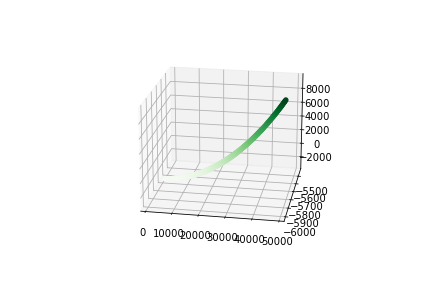
\includegraphics[width=\linewidth, height=6cm]{vs1.png} \caption{velocity} \label{vs1} \par
		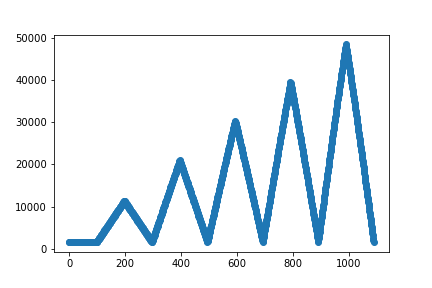
\includegraphics[width=\linewidth, height=6cm]{vsx1.png} \caption{$x$-component of velocity} \label{vsx1} \par
	\end{multicols}
\end{figure}
\begin{figure}[H]
	\begin{multicols}{2}
		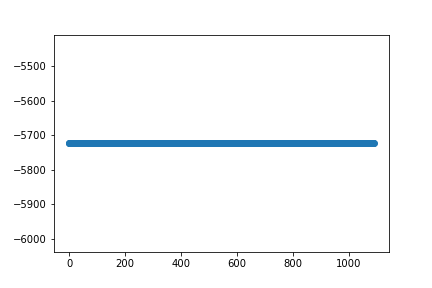
\includegraphics[width=\linewidth, height=6cm]{vsy1.png} \caption{$y$-component of velocity} \label{vsy1} \par
		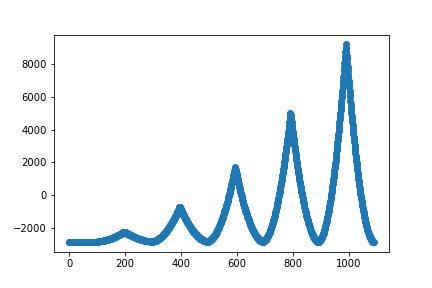
\includegraphics[width=\linewidth, height=6cm]{vsz1.png} \caption{$z$-component of velocity} \label{vsz1} \par
	\end{multicols}
\end{figure}	

\begin{tcolorbox}[width=3cm]
	$\mathbf{E} \times \mathbf{B}$ drift
\end{tcolorbox}
	$\mathbf{E} \times \mathbf{B}$ drift is the drift of a particle in direction perpendicular to the electric and the magnetic fields, which is along the $z$-axis in this example. We can see the effect of $\mathbf{E} \times \mathbf{B}$ drift in figure(\ref{ps1}) and figure(\ref{psz1}), although we also see the effect of particle having a non-zero initial velocity in some direction. What we see in figure(\ref{ps1}) which is perhaps more clear in figure(\ref{psz1}) is that the particle is initially moving downwards along the $z$-axis. But following events of changing the sign of the electric field, the particle moves upwards until the next event of the change of sign of the electric field. As the strength of the electric field becomes greater later along the update, we see that the drifts cover longer distances.
	
	In figure (\ref{vsz1}) we also see the effect of $\mathbf{E} \times \mathbf{B}$ drift, as the velocity of the particle along the direction perpendicular to the electric and magnetic field changes when we change the direction of the electric field. It seems like the $z$-component of the acceleration might have sudden discontinuities and one might expect the change in direction of the electric field  to affect the $\mathbf{E} \times \mathbf{B}$ drift. In figure (\ref{vsx1}) we see that the changes are sharp when we change the sign of the electric field. As we increase the strength of the electric field, we observe that the velocities increase to greater values. \\
	
	\noindent \textbf{!!} We should be \textbf{careful} that figure(\ref{vs1}) hides the fact that the velocity is increasing and decreasing when we change the direction of the electric field, the points in the figure overlap and we do not see the distinction between multiple instances during the update when the same velocity is attained. Figures (\ref{vsx1}) and (\ref{vsz1}) help us understand this better. We also observe in figure (\ref{vsy1}) that the $y$-component of the velocity; along the magnetic field, stays constant.
	
	A thing to notice is that we started by saying that we might want to consider a cube of size 1m x 1m x 1m; which would be a reasonable size for a plasma chamber, and we see that the particle stays well within the box. This means that such a time frame of plasma control might be relevant to processes in surface engineering where particles in hot plasma have some high velocity and participate in the processes in timescales of microseconds as in the example. 

\begin{tcolorbox}
	Animations have been generated for all plots and they help us understand these update histories better. 
\end{tcolorbox}	
	Animations were generated using the following parts of the program.
\begin{minted}[
	frame=lines,
	framesep=2mm,
	baselinestretch=1.2,
	bgcolor=LightGray,
	fontsize=\footnotesize,
	linenos=true,
	breaklines
	]
	{python}
def plot_animation_3d(positions):
	'''
	This function can plot both positions and velocities
	'''
	
	FRAMES = np.shape(positions)[0]
	# Here positions has shape (number of particles, 3) where each entry is a position which is an array of x,y,z coordinates
	fig = plt.figure()
	ax = fig.add_subplot(111, projection='3d')
	
	def init():
		ax.view_init(elev=10., azim=0)
		ax.set_xlabel('x')
		ax.set_ylabel('y')
		ax.set_zlabel('z')
	
	# animation function.  This is called sequentially
	def animate(i):
		current_index = int(positions.shape[0] / FRAMES * i)
		ax.cla()
		ax.view_init(elev=10., azim=i)
		ax.set_xlabel('x')
		ax.set_ylabel('y')
		ax.set_zlabel('z')
		# For line plot uncomment the following line
		# ax.plot3D(positions[:current_index, 0], positions[:current_index, 1], positions[:current_index, 2])
		ax.scatter3D(positions[:current_index, 0], positions[:current_index, 1], positions[:current_index, 2])
		
		# call the animator.
		anim = animation.FuncAnimation(fig, animate, init_func=init, frames=FRAMES, interval=100)
		
		return anim

def plot_animation_1d(positions, include):
	'''
	This function can plot both positions and velocities
	include can be 0, 1 or 2.
	if include = 2, this means plot the z data of the array
	'''
	
	FRAMES = np.shape(positions)[0]
	# Here positions has shape (number of particles, 3) where each entry is a position which is an array of x,y,z coordinates
	fig = plt.figure()
	ax = fig.add_subplot(111)
	
	def init():
		ax.set_xlabel('step')
		ax.set_ylabel(chr(include + 120))
	
	# animation function.  This is called sequentially
	def animate(i):
		current_index = int(positions.shape[0] / FRAMES * i)
		ax.cla()
		ax.set_xlabel('step')
		ax.set_ylabel(chr(include + 120))
		# For line plot uncomment the following line
		# ax.plot3D(positions[:current_index, 0], positions[:current_index, 1], positions[:current_index, 2])
		ax.scatter(np.arange(len(positions))[:current_index], positions[:current_index, include])
		
		# call the animator.
		anim = animation.FuncAnimation(fig, animate, init_func=init, frames=FRAMES, interval=100)

		return anim
\end{minted}

	Running the animation generation.
	

\begin{minted}[
	frame=lines,
	framesep=2mm,
	baselinestretch=1.2,
	bgcolor=LightGray,
	fontsize=\footnotesize,
	linenos=true,
	breaklines
	]
	{python}
# animation for the position of the particle
s1_allfield_p0_ps_anim = plot_animation_3d(s1_allfield_p0_ps)
display_animation(s1_allfield_p0_ps_anim)
s1_allfield_p0_ps_anim.save(r'ps1.mp4')

# x positions
s1_allfield_p0_ps_x_anim = plot_animation_1d(s1_allfield_p0_ps, include=0)
display_animation(s1_allfield_p0_ps_x_anim)
s1_allfield_p0_ps_x_anim.save(r'psx1.mp4')

# y positions
s1_allfield_p0_ps_y_anim = plot_animation_1d(s1_allfield_p0_ps, include=1)
display_animation(s1_allfield_p0_ps_y_anim)
s1_allfield_p0_ps_y_anim.save(r'psy1.mp4')

# z positions
s1_allfield_p0_ps_z_anim = plot_animation_1d(s1_allfield_p0_ps, include=2)
display_animation(s1_allfield_p0_ps_z_anim)
s1_allfield_p0_ps_z_anim.save(r'psz1.mp4')

# Plot the velocity
s1_allfield_p0_vs_anim = plot_animation_3d(s1_allfield_p0_vs)
display_animation(s1_allfield_p0_vs_anim)
s1_allfield_p0_vs_anim.save(r'vs1.mp4')

# Plot x velocity
s1_allfield_p0_vs_x_anim = plot_animation_1d(s1_allfield_p0_vs, include=0)
display_animation(s1_allfield_p0_vs_x_anim)
s1_allfield_p0_vs_x_anim.save(r'vsx1.mp4')

# Plot y velocity
s1_allfield_p0_vs_y_anim = plot_animation_1d(s1_allfield_p0_vs, include=1)
display_animation(s1_allfield_p0_vs_y_anim)
s1_allfield_p0_vs_y_anim.save(r'vsy1.mp4')

# Plot z velocity
s1_allfield_p0_vs_z_anim = plot_animation_1d(s1_allfield_p0_vs, include=2)
display_animation(s1_allfield_p0_vs_z_anim)
s1_allfield_p0_vs_z_anim.save(r'vsz1.mp4')	
\end{minted}

\begin{tcolorbox}
	In generating the animations for the plots, we took help from the blog post titled: \textbf{Charged Particle Trajectories in Electric and Magnetic Fields} (\cite{blog}).
\end{tcolorbox}

\begin{minted}[
	frame=lines,
	framesep=2mm,
	baselinestretch=1.2,
	bgcolor=LightGray,
	fontsize=\footnotesize,
	linenos=true,
	breaklines
	]
	{python}
VIDEO_TAG = """<video controls>
<source src="data:video/x-m4v;base64,{0}" type="video/mp4">
Your browser does not support the video tag.
</video>"""

def anim_to_html(anim):
	if not hasattr(anim, '_encoded_video'):
		f = NamedTemporaryFile(suffix='.mp4', delete=False)
		anim.save(f.name, fps=20, extra_args=['-vcodec', 'libx264', '-pix_fmt', 'yuv420p'])
		f.flush()
		video = open(f.name, "rb").read()
		f.close()
		anim._encoded_video = base64.b64encode(video).decode('utf-8')
	
	return VIDEO_TAG.format(anim._encoded_video)

def display_animation(anim):
	plt.close(anim._fig)
	return HTML(anim_to_html(anim))
\end{minted}

	
	\subsection{Multiparticle update plots}
	We can look at the position and velocity update histories of many particles. We pick 10 particles, the particles at indices [0, 10, 20, 30, 40, 50, 60, 70, 80, 90] to plot.
	
\begin{minted}[
	frame=lines,
	framesep=2mm,
	baselinestretch=1.2,
	bgcolor=LightGray,
	fontsize=\footnotesize,
	linenos=true,
	breaklines
	]
	{python}
s1_particles = [0, 10, 20, 30, 40, 50, 60, 70, 80, 90] # take particles at these indices
s1_allFieldkeys = list(s1_batch_ps_and_vs.keys())
s1_allfield_10p_ps = []
s1_allfield_10p_vs = []

for aparticle in s1_particles:
s1_allfield_ap_ps = []
s1_allfield_ap_vs = []

# Same procedure for as a single particle
for akey in s1_allFieldkeys:
	s1_histories = s1_batch_ps_and_vs[akey]

#Take aparticle
s1_ap = s1_histories[aparticle]

#Take ps and vs
for i in range(len(s1_p0)):
	s1_allfield_ap_ps.append(s1_ap[i][1])
	s1_allfield_ap_vs.append(s1_ap[i][2])
	s1_allfield_ap_ps = np.array(s1_allfield_ap_ps)
	s1_allfield_ap_vs = np.array(s1_allfield_ap_vs)
	
	s1_allfield_10p_ps.append(s1_allfield_ap_ps)
	s1_allfield_10p_vs.append(s1_allfield_ap_vs)

s1_allfield_10p_ps = np.array(s1_allfield_10p_ps)
s1_allfield_10p_vs = np.array(s1_allfield_10p_vs)

# Plot the positions
s1_allfield_10p_ps_fig = plt.figure()
s1_allfield_10p_ps_ax = plt.axes(projection='3d')
s1_allfield_10p_ps_ax.view_init(20, -80)

# Data for three-dimensional scattered points
for i in range(len(s1_particles)):
	s1_allfield_ap_ps_zdata = [elem[2] for elem in s1_allfield_10p_ps[i]] 
	s1_allfield_ap_ps_xdata = [elem[0] for elem in s1_allfield_10p_ps[i]]
	s1_allfield_ap_ps_ydata = [elem[1] for elem in s1_allfield_10p_ps[i]]
	s1_allfield_10p_ps_ax.scatter3D(s1_allfield_ap_ps_xdata, s1_allfield_ap_ps_ydata, s1_allfield_ap_ps_zdata, c=s1_allfield_p0_ps_zdata);
plt.savefig('multips1', dpi='figure', format='png')

# Plot x positions
s1_allfield_10p_ps_x_fig = plt.figure()
s1_allfield_10p_ps_x_ax = plt.axes()
for i in range(len(s1_particles)):
	s1_allfield_ap_ps_xdata = [elem[0] for elem in s1_allfield_10p_ps[i]]
	s1_allfield_10p_ps_x_ax.scatter(np.arange(len(s1_allfield_ap_ps_xdata)), s1_allfield_ap_ps_xdata);
plt.savefig('multipsx1', dpi='figure', format='png')

# Plot y positions
s1_allfield_10p_ps_y_fig = plt.figure()
s1_allfield_10p_ps_y_ax = plt.axes()
for i in range(len(s1_particles)):
	s1_allfield_ap_ps_ydata = [elem[1] for elem in s1_allfield_10p_ps[i]]
	s1_allfield_10p_ps_y_ax.scatter(np.arange(len(s1_allfield_ap_ps_ydata)), s1_allfield_ap_ps_ydata);
plt.savefig('multipsy1', dpi='figure', format='png')

# Plot z positions
s1_allfield_10p_ps_z_fig = plt.figure()
s1_allfield_10p_ps_z_ax = plt.axes()
for i in range(len(s1_particles)):
	s1_allfield_ap_ps_zdata = [elem[2] for elem in s1_allfield_10p_ps[i]].
	s1_allfield_10p_ps_z_ax.scatter(np.arange(len(s1_allfield_ap_ps_zdata)), s1_allfield_ap_ps_zdata);
plt.savefig('multipsz1', dpi='figure', format='png')
\end{minted}
	
	We get the following plots of the positions:
	
	\begin{figure}[H]
		\begin{multicols}{2}
			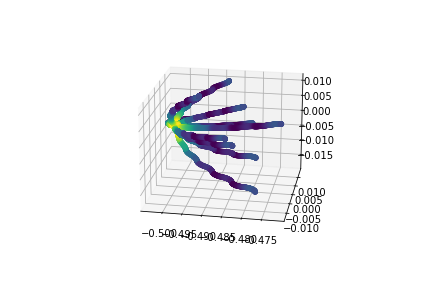
\includegraphics[width=\linewidth, height=6cm]{multips1.png} \caption{positions} \label{multips1} \par
			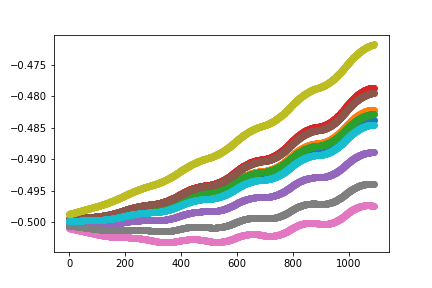
\includegraphics[width=\linewidth, height=6cm]{multipsx1.png} \caption{$x$-component of positions} \label{multipsx1} \par
		\end{multicols}
	\end{figure}
	\begin{figure}[H]
		\begin{multicols}{2}
			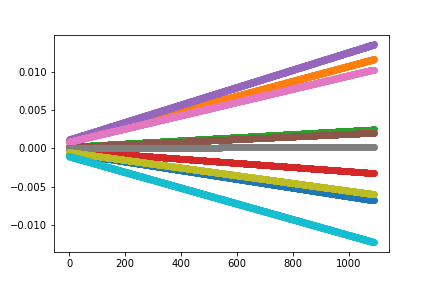
\includegraphics[width=\linewidth, height=6cm]{multipsy1.png} \caption{$y$-component of positions} \label{multipsy1} \par
			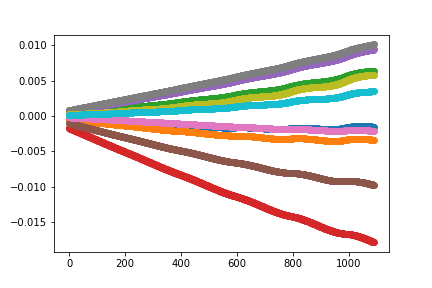
\includegraphics[width=\linewidth, height=6cm]{multipsz1.png} \caption{$z$-component of positions} \label{multipsz1} \par
		\end{multicols}
	\end{figure}
	
	In figure (\ref{multips1}), we observe that all the particles begin at the same point and spread out based on their velocities. In figures (\ref{multipsx1}), (\ref{multipsy1}) and (\ref{multipsz1}), we see that all the particles start at position [-0.5, 0, 0] as we intended them to when setting up the study; and spread out based on their initial velocities.
	
	We can also look at the velocities.
	
\begin{minted}[
	frame=lines,
	framesep=2mm,
	baselinestretch=1.2,
	bgcolor=LightGray,
	fontsize=\footnotesize,
	linenos=true,
	breaklines
	]
	{python}
# Plot the velocities
s1_allfield_10p_vs_fig = plt.figure()
s1_allfield_10p_vs_ax = plt.axes(projection='3d')
s1_allfield_10p_vs_ax.view_init(20, -120)

# Data for three-dimensional scattered points
for i in range(len(s1_particles)):
	s1_allfield_ap_vs_zdata = [elem[2] for elem in s1_allfield_10p_vs[i]] # Animate this plot as well.
	s1_allfield_ap_vs_xdata = [elem[0] for elem in s1_allfield_10p_vs[i]]
	s1_allfield_ap_vs_ydata = [elem[1] for elem in s1_allfield_10p_vs[i]]
	s1_allfield_10p_vs_ax.scatter3D(s1_allfield_ap_vs_xdata, s1_allfield_ap_vs_ydata, s1_allfield_ap_vs_zdata,\
	c=s1_allfield_p0_vs_zdata);
plt.savefig('multivs1', dpi='figure', format='png')

# Plot x velocities
s1_allfield_10p_vs_x_fig = plt.figure()
s1_allfield_10p_vs_x_ax = plt.axes()
for i in range(len(s1_particles)):
	s1_allfield_ap_vs_xdata = [elem[0] for elem in s1_allfield_10p_vs[i]]
	s1_allfield_10p_vs_x_ax.scatter(np.arange(len(s1_allfield_ap_vs_xdata)), s1_allfield_ap_vs_xdata);
plt.savefig('multivsx1', dpi='figure', format='png')

# Plot y velocities
s1_allfield_10p_vs_y_fig = plt.figure()
s1_allfield_10p_vs_y_ax = plt.axes()
for i in range(len(s1_particles)):
	s1_allfield_ap_vs_ydata = [elem[1] for elem in s1_allfield_10p_vs[i]]
	s1_allfield_10p_vs_y_ax.scatter(np.arange(len(s1_allfield_ap_vs_ydata)), s1_allfield_ap_vs_ydata);
plt.savefig('multivsy1', dpi='figure', format='png')

# Plot z velocities
s1_allfield_10p_vs_z_fig = plt.figure()
s1_allfield_10p_vs_z_ax = plt.axes()
for i in range(len(s1_particles)):
	s1_allfield_ap_vs_zdata = [elem[2] for elem in s1_allfield_10p_vs[i]]
	s1_allfield_10p_vs_z_ax.scatter(np.arange(len(s1_allfield_ap_vs_zdata)), s1_allfield_ap_vs_zdata);
plt.savefig('multivsz1', dpi='figure', format='png')
\end{minted}
	
	We get the following plots for the velocities:
\begin{figure}[H]
	\begin{multicols}{2}
		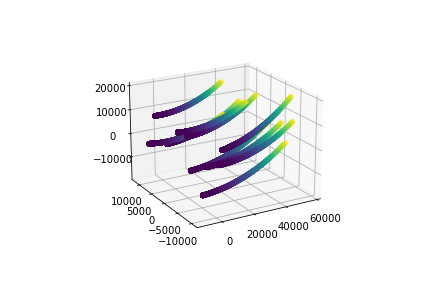
\includegraphics[width=\linewidth, height=6cm]{multivs1.png} \caption{velocities} \label{multivs1} \par
		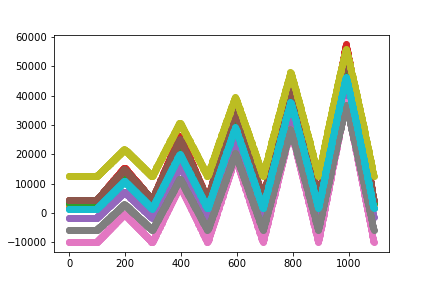
\includegraphics[width=\linewidth, height=6cm]{multivsx1.png} \caption{$x$-component of velocities} \label{multivsx1} \par
	\end{multicols}
\end{figure}
\begin{figure}[H]
	\begin{multicols}{2}
		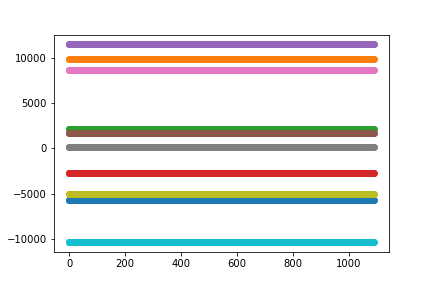
\includegraphics[width=\linewidth, height=6cm]{multivsy1.png} \caption{$y$-component of velocities} \label{multivsy1} \par
		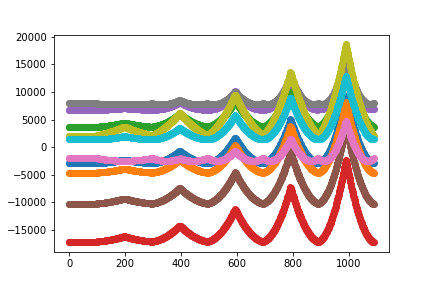
\includegraphics[width=\linewidth, height=6cm]{multivsz1.png} \caption{$z$-component of velocities} \label{multivsz1} \par
	\end{multicols}
\end{figure}	
	
	We see that the particles start out with different values for each component and the $y$-component of the velocities of the particles stay the same. Like for a single particle, we also see the effect of changing the direction of the Electric field on the $x$ and $z$ components of the velocities. Also like the single particle plots, we see that the velocity oscillations observed in figures (\ref{multivsx1}) and (\ref{multivsz1}) are not observed in figure (\ref{multivs1}) because the points in the plot overlap. Animations of the plots might help us better understand the plots. Animations were generated using the following part of the program.
	
 \begin{minted}[
 	frame=lines,
 	framesep=2mm,
 	baselinestretch=1.2,
 	bgcolor=LightGray,
 	fontsize=\footnotesize,
 	linenos=true,
 	breaklines
 	]
 	{python}
def multiplot_animation_3d(positions):
	'''
	Here each element of positions is data for 1 particle that one would give as input to
	plot_animation_3d function, i.e. position or velocity update history of 1 particle
	
	This function can plot both positions and velocities
	'''
	
	#positions = np.array(np.array([xdata, ydata, zdata]))
	FRAMES = np.shape(positions)[1]
	# Here positions has shape (10, 1089, 3) 
	fig = plt.figure()
	ax = fig.add_subplot(111, projection='3d')
	
	def init():
		ax.view_init(elev=20., azim=0)
		ax.set_xlabel('x')
		ax.set_ylabel('y')
		ax.set_zlabel('z')
	
	# animation function.  This is called sequentially
	def animate(i):
		current_index = int(positions.shape[1] / FRAMES * i)
		ax.cla()
		ax.view_init(elev=20., azim=i)
		ax.set_xlabel('x')
		ax.set_ylabel('y')
		ax.set_zlabel('z')
		# For line plot uncomment the following line
		# ax.plot3D(positions[:current_index, 0], positions[:current_index, 1], positions[:current_index, 2])
		for position in positions:
		ax.scatter3D(position[:current_index, 0], position[:current_index, 1], position[:current_index, 2])
	
		# call the animator.
		anim = animation.FuncAnimation(fig, animate, init_func=init, frames=FRAMES, interval=100)
		
		return anim
		
def multiplot_animation_1d(positions, include):
	'''Here each element of positions is data for 1 particle that one would give as input to
	plot_animation_3d function, i.e. position or velocity update history of 1 particle
	
	This function can plot both positions and velocities
	include can be 0, 1 or 2.
	if include = 2, this means plot the z data of the array
	'''
	
	#positions = np.array(np.array([xdata, ydata, zdata]))
	FRAMES = np.shape(positions)[1]
	# Here positions has shape (10, 1089, 3) 
	fig = plt.figure()
	ax = fig.add_subplot(111)
	
	def init():
		ax.set_xlabel('step')
		ax.set_ylabel(chr(include + 120))
		
	# animation function.  This is called sequentially
	def animate(i):
		current_index = int(positions.shape[1] / FRAMES * i)
		ax.cla()
		ax.set_xlabel('step')
		ax.set_ylabel(chr(include + 120))
		# For line plot uncomment the following line
		# ax.plot3D(positions[:current_index, 0], positions[:current_index, 1], positions[:current_index, 2])
		for position in positions:
		ax.scatter(np.arange(len(position))[:current_index], position[:current_index, include])
		
		# call the animator.
		anim = animation.FuncAnimation(fig, animate, init_func=init, frames=FRAMES, interval=100)
		
		return anim
 \end{minted}

	Running the animation generation.

\begin{minted}[
	frame=lines,
	framesep=2mm,
	baselinestretch=1.2,
	bgcolor=LightGray,
	fontsize=\footnotesize,
	linenos=true,
	breaklines
	]
	{python}
# Animate the positions
s1_allfield_10p_ps_anim = multiplot_animation_3d(s1_allfield_10p_ps)
display_animation(s1_allfield_10p_ps_anim)
s1_allfield_10p_ps_anim.save(r'multips1.mp4')

# x positions
s1_allfield_10p_ps_x_anim = multiplot_animation_1d(s1_allfield_10p_ps, include=0)
display_animation(s1_allfield_10p_ps_x_anim)
s1_allfield_10p_ps_x_anim.save(r'multipsx1.mp4')

# y positions
s1_allfield_10p_ps_y_anim = multiplot_animation_1d(s1_allfield_10p_ps, include=1)
display_animation(s1_allfield_10p_ps_y_anim)
s1_allfield_10p_ps_y_anim.save(r'multipsy1.mp4')

# z positions
s1_allfield_10p_ps_z_anim = multiplot_animation_1d(s1_allfield_10p_ps, include=2)
display_animation(s1_allfield_10p_ps_z_anim)
s1_allfield_10p_ps_z_anim.save(r'multipsz1.mp4')

# Animate the velocities
s1_allfield_10p_vs_anim = multiplot_animation_3d(s1_allfield_10p_vs)
display_animation(s1_allfield_10p_vs_anim)
s1_allfield_10p_vs_anim.save(r'multivs1.mp4')

# x velocities
s1_allfield_10p_vs_x_anim = multiplot_animation_1d(s1_allfield_10p_vs, include=0)
display_animation(s1_allfield_10p_vs_x_anim)
s1_allfield_10p_vs_x_anim.save(r'multivsx1.mp4')

#y velocities
s1_allfield_10p_vs_y_anim = multiplot_animation_1d(s1_allfield_10p_vs, include=1)
display_animation(s1_allfield_10p_vs_y_anim)
s1_allfield_10p_vs_y_anim.save(r'multivsy1.mp4')

# z velocities
s1_allfield_10p_vs_z_anim = multiplot_animation_1d(s1_allfield_10p_vs, include=2)
display_animation(s1_allfield_10p_vs_z_anim)
s1_allfield_10p_vs_z_anim.save(r'multivsz1.mp4')
\end{minted}

	In this first simple study, we were able to look at the behavior of a system of particles being updated under the influence of non-uniform electric field. In particular, we were able to observe the $\mathbf{E} \times \mathbf{B}$ drift. Next, we will use the radial electric field function that we have defined; intended to mimic the electric field generated due to an electrode, and the helmholtz magnetic field generated by Helmholtz coils. 
	
	\subsection{Other field configurations}
		\color{red}
	\begin{itemize}
		\item Change Voltage of electrode to change electric field
		\item Change current in Helmholtz coil to change the magnetic field 
	\end{itemize}
	while the updates are running.
	on different batches.
	\color{black}	\\ 
	
	\section{The Magnetic Mirror configuration}
	\color{red}
	\textbf{need parabolic $\mathbf{B}$ along $z$-axis configuration for $\nabla$$\mathbf{B}$ $\parallel$ $\mathbf{B}$ }
	
	\begin{itemize}
		\item Maxwellian distribution
		\item maybe Parabolic distribution
	\end{itemize}
	\color{black}
	
	\begin{thebibliography}{}
		\bibitem{blog} Florian LB (GitHub user). \textit{Charged Particle Trajectories in Electric and Magnetic Fields}. Thu, 28 Jan 2016. \textit{https://flothesof.github.io/charged-particle-trajectories-E-and-B-fields.html}
	\end{thebibliography}
\end{document}